\part{SW 02 - ISO/OSI Modell}
\section{Lernziele (Leitfragen)}
\begin{enumerate}
    \item Was sind die Schichten des TCP/IP Models? Beschreiben Sie den Zweck jeder Schicht
    \item Was sind die Schichten des OSI Models? Beschreiben Sie den Zweck jeder Schicht
    \item Was ist die Verbindung zwischen dem TCP/IP Modell und dem OSI Modell?
    \item Nehmen Sie eine typische Netzwerkapplikation als Beispiel. Anhand des TCP/IP Models, erläutern Sie wie Nachrichten zwischen den End-Devices ausgetauscht sind.
    \item Wieso muss man Zahlensysteme verstehen, wenn man sich mit Computernetzwerken beschäftigt?
    \item Wie kann man einfach und schnell zwischen Binär, Hexadezimal und Dezimal umrechnen?
\end{enumerate}

\section{Antworten}
\subsection*{Was sind die Schichten des TCP/IP Models? Beschreiben Sie den Zweck jeder Schicht}
Das TCP/IP Modell besteht aus vier Schichten.\\

\begin{table}[H]
\begin{tabularx}{\textwidth}{|c|X|l|}
    \multicolumn{1}{c}{Layer}&\multicolumn{1}{X}{Zusammenfassung}&\multicolumn{1}{l}{Protokolle}\\
    \hline
    \makecell[c]{Application}&\makecell[X]{- Am nächsten zum User\\- Datenaustausch zwischen Programmen\\- Allgemeine Funktionen zur Kommunikation im Internet}&\makecell[l]{Web (HTTP, HTTPS)\\Email (POP, IMAP, SMTP)\\Namensauflösung (DNS)\\Datenaustausch (FTP)}\\
    \hline
    \makecell{Transport}&\makecell[X]{- Segmentierung und Zusammenfügen von Daten\\- Management von Verlässlichkeitsanforderungen einer Konversation\\- Multiplexing und Konversationen verfolgen}&\makecell[l]{Verbindungsorierntiert (TCP)\\Verbindungslos (UDP)}\\
    \hline
    \makecell{Internet}&\makecell[X]{- Datenaustausch über Sub-Netzwerke\\- Adressierung von Endgeräten\\- Routing\\- verbindungslos, best effort und medienunabhängig}&\makecell[l]{Datenaustausch (IPv4, IPv6)\\Routing (OSPF, BGP)\\Steuerung (ICMPv4, ICMPv6)}\\
    \hline
    \makecell{Network\\Access}&\makecell[X]{- Adressierung von Sub-Netzwerken\\- Media access control (MAC)\\- Abstraktion der physischen Medien der oberen Schichten\\- Bits auf die Medien setzen}&\makecell[l]{Address Resolution (ARP)\\Data Link (Ethernet, WLAN)}\\
    \hline
\end{tabularx}
\caption{TCP/IP Modell}
\end{table}
\subsection*{Was sind die Schichten des OSI Models? Beschreiben Sie den Zweck jeder Schicht}
Das OSI Modell besteht aus 7 Schichten.\\
//TODO
\begin{table}[H]
\begin{tabularx}{\textwidth}{|cc|X|l|}
    \multicolumn{2}{c}{Layer}&\multicolumn{1}{X}{Zusammenfassung}&\multicolumn{1}{l}{Protokolle}\\
    \hline
    7&Anwendungen&blub&DHCP\\
    &(Application)&blub&HTTP\\
    \hline
\end{tabularx}
\caption{OSI Modell}
\end{table}
\subsection*{Was ist die Verbindung zwischen dem TCP/IP Modell und dem OSI Modell?}
\begin{figure}[H]
    \begin{center}
    \label{pic:osi_tcpip}
    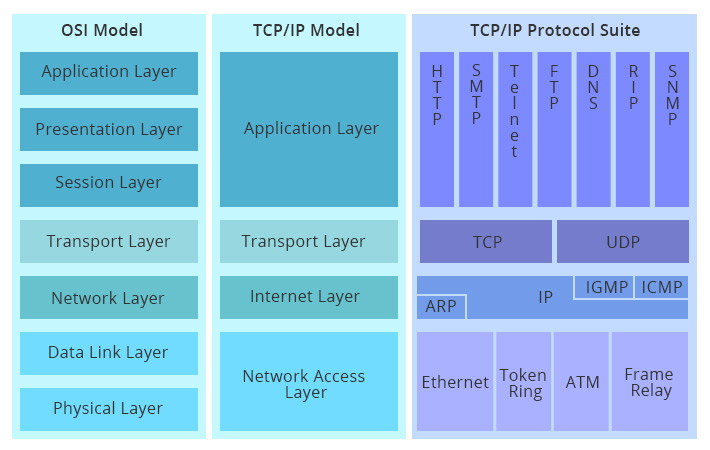
\includegraphics[width=\textwidth]{images/osi_tcpip.jpg}
    \caption[Vergleich OSI mit TCP/IP Modell]{Vergleich OSI mit TCP/IP Modell\footnotemark}
    \end{center}
\end{figure}
\footnotetext{\url{https://media.fs.com/images/community/wp-content/uploads/2017/11/comparison-of-OSI-and-TCPIP.jpg}}
\subsection*{Nehmen Sie eine typische Netzwerkapplikation als Beispiel. Anhand des TCP/IP Models, erläutern Sie wie Nachrichten zwischen den End-Devices ausgetauscht sind.}
//TODO
\subsection*{Wieso muss man Zahlensysteme verstehen, wenn man sich mit Computernetzwerken beschäftigt?}
//TODO
\subsection*{Wie kann man einfach und schnell zwischen Binär, Hexadezimal und Dezimal umrechnen?}
    Über den Rechner vom Betriebssystem:
    \begin{figure}[H]
        \begin{center}
        \label{pic:calc}
        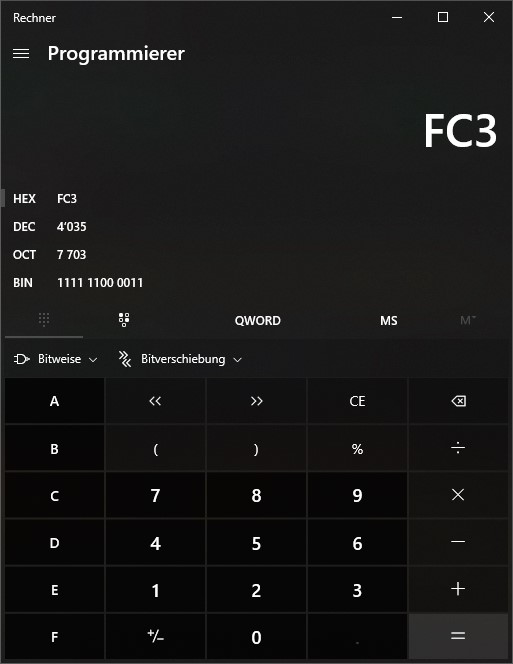
\includegraphics[width=.5\textwidth]{images/calc.jpg}
        \caption{Windows Taschenrechner}
        \end{center}
    \end{figure}
    Oder ganz easy von Hand ausrechnen.
    \paragraph{Binär}Beispiel 125 zu Binär. Den Rest zusammenfügen:\\
    \begin{tabular}{rll}
        125:&2 = 62&R 1 (ganz rechts)\\
        62:&2 = 31&R 0\\
        31:&2 = 15&R 1\\
        15:&2 = 7&R 1\\
        7:&2 = 3&R 1\\
        3:&2 = 1&R 1\\
        1:&2 = 0&R 1 (ganz links)\\[1em]
\end{tabular}
Dann ist das Ergebnis also: 0b111 1101\\[1em]
Um die Binärzahl in Dezimal umzuwandeln, liest man von rechts die Einsen und fängt mit der Potenz 0 zur Basis 2 an. Unser Zahlenbeispiel als Byte:\\[1em]
\begin{tabular}{cccccccc}
    $2^7$&$2^6$&$2^5$&$2^4$&$2^3$&$2^2$&$2^1$&$2^0$\\
    0&1&1&1&1&1&0&1\\
\end{tabular}\\[1em]
Daraus erhält man, dort wo eine 1 steht:\\$2^6+2^5+2^4+2^3+2^2+2^0=64+32+16+8+4+1=125$.

\paragraph{Hexadezimal}Hexadezimal ist da schon etwas komplizierter, aber machbar. Hier rechnet man auch mit Potenzen zur Basis 16. Dazu muss man vorgängig aber schon das $16^x$ unterhalb der Zahl kennen.\\
$16^2=256$ ist also zu hoch für unsere 125. Bleibt also die nächst tiefere Potenz  $16^1=16$.\\
Wir teilen also mit 16:\\
\begin{tabular}{rllll}
    125:&16&($16^1$)&= 7 (ganz links)&R  13 (mit nächst tiefere Potenz teilen)\\
    13:&1&($16^0$) &= 13&\\[1em]
\end{tabular}\\
Also hat man jetzt $7\times16^1+13\times16^0$. Das Hexadezimalsystem geht ja aber von 0-F, somit ist die 13 ein D (\dots, 9, 10=A, 11=B, 12=C, 13=D, 14=E, 15=F). Das Ergebnis ist als 0x7D. Auch easy.\\
Umgekehrt von Hexadezimal auf Dezimal umzurechnen, folgt man dem nun bekannten Potenz-Prinzip.\\
Hexadezimal und Binär ist Bubieinfach. Dazu nimmt man Binär halbe Bytes und stellt die Zahlen gegenüber.\\
\begin{tabular}{cccc|cccc}
    $2^3$&$2^2$&$2^1$&$2^0$&$2^3$&$2^2$&$2^1$&$2^0$\\
    0&1&1&1&1&1&0&1\\
    \hline
    \multicolumn{4}{c|}{7}&\multicolumn{4}{c}{13 = D}\\
\end{tabular}
